% Mars H2 upper boundary conditions (Kepler hold vs explicit RK4) compared with Carberry Mogan et al. (2021).
% Build (from this folder):  tectonic -o build main.tex
% Every number set in mono comes from numbers.tex or tables/*.tex (scripts/make_numbers.py);
% figures come from scripts/make_figures.py. Design: design_philosophy.md ("Graphite Telemetry").
% Data: analysis-tier files written by campaigns/h2_hold and campaigns/h2_ubc_rtop (docs/CONVENTIONS.md).
\documentclass[10pt]{article}

% ------------------------------------------------------------------ page
\usepackage[letterpaper,margin=1in,headheight=14pt,headsep=18pt,footskip=28pt]{geometry}
\usepackage[parfill]{parskip}
\setlength{\parskip}{5pt plus 1pt}

% ------------------------------------------------------------------ type
\usepackage{fontspec}
\usepackage{unicode-math}
\defaultfontfeatures{Ligatures=TeX}
\setmainfont{InstrumentSans}[
  Path=fonts/, Extension=.ttf,
  UprightFont=*-Regular, BoldFont=*-Bold, ItalicFont=*-Italic, BoldItalicFont=*-BoldItalic,
  Numbers=Tabular]
\setsansfont{InstrumentSans}[
  Path=fonts/, Extension=.ttf,
  UprightFont=*-Regular, BoldFont=*-Bold, ItalicFont=*-Italic, BoldItalicFont=*-BoldItalic]
\setmonofont{JetBrainsMono}[
  Path=fonts/, Extension=.ttf, UprightFont=*-Regular, BoldFont=*-Bold, Scale=0.86, HyphenChar=None]
\setmathfont{FiraMath-Regular.otf}
\linespread{1.13}
\setlength{\emergencystretch}{1.5em}
\widowpenalty=10000
\clubpenalty=10000
\usepackage{microtype}

% ------------------------------------------------------------------ inks
\usepackage[table]{xcolor}
\definecolor{charcoal}{HTML}{1F1F1D}
\definecolor{graphite}{HTML}{4A4A47}
\definecolor{grey}{HTML}{7A7A76}
\definecolor{lightgrey}{HTML}{B9B8B3}
\definecolor{rulegrey}{HTML}{E6E5E1}
\definecolor{inkO}{HTML}{2A78D6}
\definecolor{inkH}{HTML}{EB6834}

% ------------------------------------------------------------------ floats, tables
\usepackage{graphicx}
\graphicspath{{figures/}}
\usepackage{booktabs}
\usepackage{float}
\usepackage{tabularx}
\usepackage{array}
\arrayrulecolor{lightgrey}
\setlength{\heavyrulewidth}{0.6pt}
\setlength{\lightrulewidth}{0.4pt}
\setlength{\cmidrulewidth}{0.4pt}
\renewcommand{\arraystretch}{1.18}
\usepackage{caption}
\DeclareCaptionFont{graphite}{\color{graphite}}
\DeclareCaptionFont{charcoal}{\color{charcoal}}
\captionsetup{font={small,graphite}, labelfont={bf,charcoal}, labelsep=quad,
  justification=raggedright, singlelinecheck=false, skip=6pt}
\captionsetup[table]{position=top, skip=4pt}
\setlength{\textfloatsep}{16pt plus 4pt minus 2pt}
\setlength{\floatsep}{14pt plus 4pt minus 2pt}
\renewcommand{\topfraction}{0.9}
\renewcommand{\textfraction}{0.08}
\renewcommand{\floatpagefraction}{0.8}

% ------------------------------------------------------------------ headings
\usepackage{titlesec}
\titleformat{\section}{\normalfont\fontsize{12.5}{16}\selectfont\bfseries}
  {\textcolor{grey}{\ttfamily\mdseries\thesection}}{0.9em}{}
\titlespacing*{\section}{0pt}{16pt plus 3pt}{4pt}
\titleformat{\subsection}{\normalfont\fontsize{10}{13}\selectfont\bfseries}
  {\textcolor{grey}{\ttfamily\mdseries\thesubsection}}{0.8em}{}
\titlespacing*{\subsection}{0pt}{10pt plus 2pt}{2pt}
\newcommand{\para}[1]{\textbf{#1}\hspace{0.5em}}

% ------------------------------------------------------------------ date
\newcommand{\twodigit}[1]{\ifnum#1<10 0\fi\number#1}
\newcommand{\reportdate}{\number\year-\twodigit{\month}-\twodigit{\day}}

% ------------------------------------------------------------------ header / footer
\usepackage{fancyhdr}
\pagestyle{fancy}
\fancyhf{}
\renewcommand{\headrulewidth}{0pt}
\fancyhead[L]{\footnotesize\color{grey}Mars H\textsubscript{2} upper boundary conditions \enspace·\enspace internal report}
\fancyhead[R]{\footnotesize\color{grey}\ttfamily v1.0 · \reportdate}
\fancyfoot[R]{\footnotesize\color{grey}\ttfamily\thepage}
\fancypagestyle{plain}{\fancyhf{}\fancyfoot[R]{\footnotesize\color{grey}\ttfamily\thepage}}

% ------------------------------------------------------------------ boxes, links, citations
\usepackage[most]{tcolorbox}
\usepackage{enumitem}
\setlist{itemsep=2pt, topsep=2pt, parsep=0pt, leftmargin=1.3em}
\setlist[itemize]{label={\color{grey}–}}
\usepackage[round,authoryear]{natbib}
\setlength{\bibsep}{3pt}
\usepackage[hidelinks]{hyperref}
\hypersetup{pdftitle={Upper boundary conditions for H2 escape on Mars: Kepler hold vs explicit ballistic tracking},
  pdfauthor={José Pérez Chávez}}

% ------------------------------------------------------------------ numbers
\newcommand{\numfont}{\ttfamily}
\newcommand{\num}[1]{{\numfont #1}}
\newcommand{\sci}[2]{{\numfont #1×10\textsuperscript{#2}}}
\newcommand{\Htwo}{H\textsubscript{2}}
\newcommand{\sinv}{s\textsuperscript{−1}}
\newcommand{\minv}{m\textsuperscript{−3}}
\newcommand{\unit}[1]{\,#1}
% Placeholder for values whose inputs are still running (written by make_numbers.py).
\newcommand{\pending}[1]{{\color{grey}\ttfamily [pending:~#1]}}
% Short form for wide tables; the caption states the reason.
\newcommand{\shortpending}{\renewcommand{\pending}[1]{{\color{grey}\ttfamily [pending]}}}
\newcommand{\torb}{t_\mathrm{orb}}
\newcommand{\tauf}{\tau_{90}}
\newcommand{\rtop}{r_\mathrm{top}}
\newcommand{\rhill}{r_\mathrm{Hill}}
% generated by scripts/make_numbers.py -- do not edit
% \pending{<reason>} must be defined in main.tex (see make_numbers.py docstring)
\newcommand{\TRatioCampExplicitTop}{\num{0.884}\,$\pm$\,\num{0.018}}
\newcommand{\TRatioCampKeplerTop}{\num{0.881}\,$\pm$\,\num{0.017}}
\newcommand{\TRatioExplicitTop}{\num{1.004}\,$\pm$\,\num{0.027}}
\newcommand{\TRatioFreeMaxDev}{\num{43.0}}
\newcommand{\TRatioFreeTop}{\num{0.570}\,$\pm$\,\num{0.009}}
\newcommand{\TRatioKeplerMaxDev}{\num{20.8}}
\newcommand{\TRatioKeplerTop}{\num{0.792}\,$\pm$\,\num{0.017}}
\newcommand{\TZmaxExplicit}{\num{2.3}}
\newcommand{\TZmaxFree}{\num{48.0}}
\newcommand{\TZmaxKepler}{\num{14.2}}
\newcommand{\TtopReflect}{\num{78}}
\newcommand{\TtopReflectRaw}{\num{82}}
\newcommand{\anBallisticExcess}{\num{3.3}}
\newcommand{\anBallisticOverJ}{\num{1.033}}
\newcommand{\anFreeOverJTop}{\num{2.18}}
\newcommand{\anInRetCampLow}{\num{1.001}}
\newcommand{\anInRetCampMid}{\num{1.012}}
\newcommand{\anInRetCampRange}{\num{1.001}--\num{1.104}}
\newcommand{\anInRetCampTop}{\num{1.104}}
\newcommand{\anInRetVerEnd}{\num{1.014}}
\newcommand{\anPhiRatioVer}{\num{1.033}}
\newcommand{\anReflectOverJ}{\num{1.000}}
\newcommand{\anRinVer}{\sci{3.96}{28}}
\newcommand{\belowKnZeroMaxDev}{\num{0.4}}
\newcommand{\campHeldFracAnLow}{\num{86}}
\newcommand{\campHeldFracAnMid}{\num{77}}
\newcommand{\campHeldFracAnTop}{\num{68}}
\newcommand{\campHeldOverAnalyticLow}{\num{1.28} / \num{1.28}}
\newcommand{\campHeldOverAnalyticMid}{\num{1.66} / \num{1.65}}
\newcommand{\campHeldOverAnalyticRange}{\num{1.281}--\num{1.661}}
\newcommand{\campHeldOverAnalyticTop}{\num{1.63} / \num{1.63}}
\newcommand{\campInRetLow}{\num{1.001} / \num{1.001}}
\newcommand{\campInRetMid}{\num{1.018} / \num{1.018}}
\newcommand{\campInRetRange}{\num{1.001}--\num{1.123}}
\newcommand{\campInRetTop}{\num{1.119} / \num{1.123}}
\newcommand{\campLateKs}{\num{1\,000}}
\newcommand{\campNdone}{\num{9}}
\newcommand{\campNlive}{\num{9}}
\newcommand{\campNtotal}{\num{9}}
\newcommand{\campPhiRatioPullMax}{\num{2.9}}
\newcommand{\campPhiRatioRange}{\num{0.986}--\num{1.018}}
\newcommand{\campReflectInEqRet}{yes}
\newcommand{\campRheldMaxHi}{\sci{7.39}{5}}
\newcommand{\campRheldMaxLo}{\sci{7.25}{5}}
\newcommand{\campTend}{\sci{2}{6}}
\newcommand{\campTendOverTau}{\num{0.39}}
\newcommand{\campTlast}{\sci{2.0}{6}}
\newcommand{\campViolMax}{\num{0}}
\newcommand{\campZLow}{\num{2\,500}}
\newcommand{\campZMid}{\num{10\,000}}
\newcommand{\campZTop}{\num{40\,000}}
\newcommand{\collEnhanceTop}{\num{1.42}}
\newcommand{\drEffectMax}{\num{4.6}}
\newcommand{\drSkipZtop}{\num{2\,500}}
\newcommand{\eightEntry}{\num{2.49}}
\newcommand{\eightEntrySteady}{\num{2.61}}
\newcommand{\eightGrowth}{\num{2.65}}
\newcommand{\eightHeldEnd}{\num{49\,704}}
\newcommand{\eightReturns}{\num{0}}
\newcommand{\eightTend}{\sci{2}{4}}
\newcommand{\escDriftHi}{\num{2}}
\newcommand{\escDriftLo}{\num{−4}}
\newcommand{\escLateCollEnhanceTop}{\num{1.45}}
\newcommand{\escLateReflectRange}{\num{1.39}--\num{1.55}}
\newcommand{\escLateStartKs}{\num{200}}
\newcommand{\exoKnHeightH}{\num{1.5}}
\newcommand{\exoPhiExplicitKn}{\num{1.29}}
\newcommand{\exoPhiExplicitKnZero}{\num{1.08}}
\newcommand{\exoPhiFreeKn}{\num{2.63}}
\newcommand{\exoPhiFreeKnZero}{\num{2.27}}
\newcommand{\exoPhiKeplerKn}{\num{1.27}}
\newcommand{\exoPhiKeplerKnZero}{\num{1.09}}
\newcommand{\exoPhiReflectKn}{\num{1.24}}
\newcommand{\exoPhiReflectKnZero}{\num{1.04}}
\newcommand{\exoRExplicitKn}{\num{1.140}}
\newcommand{\exoRExplicitKnZero}{\num{1.449}}
\newcommand{\exoRFreeKn}{\num{1.140}}
\newcommand{\exoRFreeKnZero}{\num{1.449}}
\newcommand{\exoRKeplerKn}{\num{1.140}}
\newcommand{\exoRKeplerKnZero}{\num{1.449}}
\newcommand{\exoRReflectKn}{\num{1.140}}
\newcommand{\exoRReflectKnZero}{\num{1.449}}
\newcommand{\exoTExplicitKn}{\num{0.997}}
\newcommand{\exoTExplicitKnZero}{\num{0.987}}
\newcommand{\exoTFreeKn}{\num{0.996}}
\newcommand{\exoTFreeKnZero}{\num{0.982}}
\newcommand{\exoTKeplerKn}{\num{0.996}}
\newcommand{\exoTKeplerKnZero}{\num{0.983}}
\newcommand{\exoTReflectKn}{\num{0.997}}
\newcommand{\exoTReflectKnZero}{\num{0.987}}
\newcommand{\exoZExplicitKn}{\num{588}}
\newcommand{\exoZExplicitKnZero}{\num{1\,666}}
\newcommand{\exoZFreeKn}{\num{588}}
\newcommand{\exoZFreeKnZero}{\num{1\,666}}
\newcommand{\exoZKeplerKn}{\num{588}}
\newcommand{\exoZKeplerKnZero}{\num{1\,665}}
\newcommand{\exoZReflectKn}{\num{588}}
\newcommand{\exoZReflectKnZero}{\num{1\,666}}
\newcommand{\generatedOn}{\texttt{2026-11-13 01:15}}
\newcommand{\heldFracCampEnd}{\num{68}}
\newcommand{\heldFracSweepEnd}{\num{28}}
\newcommand{\heldFracVerEnd}{\num{55}}
\newcommand{\heldSteadyHi}{\sci{4.39}{32}}
\newcommand{\heldSteadyLo}{\sci{1.94}{32}}
\newcommand{\keplerOverReflectRange}{\num{0.92}--\num{1.02}}
\newcommand{\nPending}{none}
\newcommand{\nRatioCampExplicitTop}{\num{0.849}\,$\pm$\,\num{0.053}}
\newcommand{\nRatioCampKeplerTop}{\num{0.859}\,$\pm$\,\num{0.055}}
\newcommand{\nRatioExplicitTop}{\num{0.988}\,$\pm$\,\num{0.067}}
\newcommand{\nRatioFreeMaxDev}{\num{45.1}}
\newcommand{\nRatioFreeTop}{\num{0.549}\,$\pm$\,\num{0.011}}
\newcommand{\nRatioKeplerMaxDev}{\num{19.9}}
\newcommand{\nRatioKeplerTop}{\num{0.820}\,$\pm$\,\num{0.028}}
\newcommand{\nSweepDone}{\num{30}}
\newcommand{\nSweepPairs}{\num{10}}
\newcommand{\nSweepTotal}{\num{30}}
\newcommand{\nZmaxExplicit}{\num{2.5}}
\newcommand{\nZmaxFree}{\num{25.2}}
\newcommand{\nZmaxKepler}{\num{6.5}}
\newcommand{\oBottomRun}{\texttt{H2\_U1\_z40000\_dr250}}
\newcommand{\oDref}{\num{2.92}}
\newcommand{\oDt}{\num{1}}
\newcommand{\oHill}{\num{311}}
\newcommand{\oHillKm}{\sci{1.08}{6}}
\newcommand{\oKnBottom}{\num{0.41}}
\newcommand{\oKnH}{\num{0.36}}
\newcommand{\oKnRatio}{\num{13}}
\newcommand{\oKnZero}{\num{0.033}}
\newcommand{\oKnZeroBottom}{\num{0.039}}
\newcommand{\oLambdaZero}{\num{11.04}}
\newcommand{\oMass}{\num{2.02}}
\newcommand{\oMfpBottom}{\num{136}}
\newcommand{\oMfpZero}{\num{115}}
\newcommand{\oNBottom}{\sci{1.93}{13}}
\newcommand{\oNzero}{\sci{2.3}{13}}
\newcommand{\oOmega}{\num{0.67}}
\newcommand{\oPhiJZero}{\sci{2.85}{26}}
\newcommand{\oRtopHi}{\num{12.5}}
\newcommand{\oRtopLo}{\num{1.72}}
\newcommand{\oRzero}{\num{3\,489.5}}
\newcommand{\oScaleHZero}{\num{316}}
\newcommand{\oTzero}{\num{270}}
\newcommand{\oWeight}{\sci{1.48}{28}}
\newcommand{\oZtopHiKm}{\num{40\,134}}
\newcommand{\oZtopLoKm}{\num{2\,627.3}}
\newcommand{\oZzero}{\num{100}}
\newcommand{\pDtHi}{\num{3}}
\newcommand{\pDtLo}{\num{0.75}}
\newcommand{\pExoKnBallistic}{\num{8.85}}
\newcommand{\pExoKnReflect}{\num{12.0}}
\newcommand{\pExoKnZeroReflect}{\num{6.14}}
\newcommand{\pFigOneKn}{\num{0.01}}
\newcommand{\pFigOneLambda}{\num{10}}
\newcommand{\pFigThreeThi}{\num{5}}
\newcommand{\pFigThreeTlo}{\num{0.75}}
\newcommand{\pHill}{\num{20.8}}
\newcommand{\pInRetEnd}{\num{1.28}}
\newcommand{\pInRetStart}{\num{2.4}}
\newcommand{\pKnZero}{\sci{2.5}{−3}}
\newcommand{\pLambdaZero}{\num{4.69}}
\newcommand{\pNzero}{\sci{4}{14}}
\newcommand{\pOverestimate}{\num{25}}
\newcommand{\pPhiJZero}{\sci{4.87}{29}}
\newcommand{\pPhiOneTorbBallistic}{\sci{1.1}{29}}
\newcommand{\pPhiOneTorbRatio}{\num{0.79}}
\newcommand{\pPhiOneTorbReflect}{\sci{1.4}{29}}
\newcommand{\pPhiRatioEnd}{\num{0.845}}
\newcommand{\pPhiRatioStart}{\num{0.73}}
\newcommand{\pRmaxHi}{\num{40}}
\newcommand{\pRmaxLo}{\num{2}}
\newcommand{\pRunTime}{\sci{7.5}{6}--\sci{3.0}{7}}
\newcommand{\pRzero}{\num{2\,410}}
\newcommand{\pTorb}{\sci{1.44}{6}}
\newcommand{\pTzero}{\num{155}}
\newcommand{\phiOverJFree}{\num{2.99}--\num{129.33}}
\newcommand{\phiOverJFreeLowZ}{\num{129.3}}
\newcommand{\phiOverJFreeLowZkm}{\num{2\,500}}
\newcommand{\phiOverJFreeTop}{\num{2.99}}
\newcommand{\phiOverJKepler}{\num{1.39}--\num{1.45}}
\newcommand{\phiOverJReflect}{\num{1.40}--\num{1.55}}
\newcommand{\prodEscRatioTop}{\num{0.993}\,$\pm$\,\num{0.006}}
\newcommand{\prodHeldRatioRange}{\num{0.992}--\num{1.006}}
\newcommand{\prodNTops}{\num{3}}
\newcommand{\prodSimReachedTop}{\sci{2.0}{6}}
\newcommand{\prodWallExplicitLow}{\num{12.2}}
\newcommand{\prodWallExplicitMid}{\num{12.5}}
\newcommand{\prodWallExplicitTop}{\num{13.8}}
\newcommand{\prodWallKeplerLow}{\num{10.2}}
\newcommand{\prodWallKeplerMid}{\num{11.4}}
\newcommand{\prodWallKeplerTop}{\num{13.2}}
\newcommand{\prodWallRatioLow}{\num{1.19}}
\newcommand{\prodWallRatioMid}{\num{1.10}}
\newcommand{\prodWallRatioRange}{\num{1.04}--\num{1.19}}
\newcommand{\prodWallRatioTop}{\num{1.04}}
\newcommand{\prodZmaxN}{\num{2.5}}
\newcommand{\prodZmaxNLow}{\num{1.5}}
\newcommand{\prodZmaxNMid}{\num{1.3}}
\newcommand{\prodZmaxNTop}{\num{2.5}}
\newcommand{\prodZmaxT}{\num{2.3}}
\newcommand{\prodZmaxTLow}{\num{0.3}}
\newcommand{\prodZmaxTMid}{\num{0.8}}
\newcommand{\prodZmaxTTop}{\num{2.3}}
\newcommand{\profTopAltKm}{\num{40\,002}}
\newcommand{\profWindowReflect}{\num{100}}
\newcommand{\profZtop}{\num{40\,000}}
\newcommand{\sweepHeldOverAnalytic}{\num{1.21}--\num{1.39}}
\newcommand{\sweepPhiRatioLateRange}{\num{0.923}--\num{1.025}}
\newcommand{\sweepPhiRatioPullMax}{\num{4.7}}
\newcommand{\sweepPhiRatioRange}{\num{0.920}--\num{1.016}}
\newcommand{\sweepPhiRatioTop}{\num{1.016}\,$\pm$\,\num{0.019}}
\newcommand{\sweepTend}{\sci{3}{5}}
\newcommand{\sweepTendOverTau}{\num{0.058}}
\newcommand{\tReturnMax}{\sci{1.21}{7}}
\newcommand{\tReturnMaxDays}{\num{140}}
\newcommand{\tReturnMaxOrb}{\num{8.4}}
\newcommand{\tauFillHi}{\sci{5.18}{6}}
\newcommand{\tauFillHiOrb}{\num{3.6}}
\newcommand{\tauFillLo}{\sci{2.97}{6}}
\newcommand{\tauFillLoOrb}{\num{2.1}}
\newcommand{\verDTMaxExplicit}{\num{1.16}}
\newcommand{\verDTMaxKepler}{\num{1.06}}
\newcommand{\verDTMaxReflect}{\num{0.27}}
\newcommand{\verDelayMean}{\num{0.501}}
\newcommand{\verDelayStd}{\num{0.288}}
\newcommand{\verDelayUniformStd}{\num{0.289}}
\newcommand{\verDnMaxExplicit}{\num{0.73}}
\newcommand{\verDnMaxKepler}{\num{0.42}}
\newcommand{\verDnMaxReflect}{\num{0.22}}
\newcommand{\verEscKExplicit}{\num{601}}
\newcommand{\verEscKKepler}{\num{595}}
\newcommand{\verEscKReflect}{\num{546}}
\newcommand{\verEscRatioExplicit}{\num{1.006}}
\newcommand{\verEscRatioKepler}{\num{0.996}}
\newcommand{\verEscRatioReflect}{\num{0.945}}
\newcommand{\verEscZExplicit}{\num{0.2}}
\newcommand{\verEscZKepler}{\num{−0.1}}
\newcommand{\verEscZReflect}{\num{−1.3}}
\newcommand{\verHalfDt}{\num{0.5}}
\newcommand{\verHeldRatioExplicit}{\num{1.003}}
\newcommand{\verHeldRatioKepler}{\num{0.996}}
\newcommand{\verInRetExplicit}{\num{1.018}}
\newcommand{\verInRetKepler}{\num{1.019}}
\newcommand{\verKvsEHeld}{\num{0.71}}
\newcommand{\verKvsEZ}{\num{2.8}}
\newcommand{\verNHoldRuns}{\num{6}}
\newcommand{\verPhiRatioExplicit}{\num{1.101}\,$\pm$\,\num{0.065}}
\newcommand{\verPhiRatioKepler}{\num{1.090}\,$\pm$\,\num{0.065}}
\newcommand{\verRestartHeld}{\num{0.9}}
\newcommand{\verRestartZ}{\num{0.8}}
\newcommand{\verRheldMax}{\sci{7.98}{4}}
\newcommand{\verTend}{\sci{6}{4}}
\newcommand{\verTendRestart}{\sci{3}{4}}
\newcommand{\verTendShort}{\sci{2}{4}}
\newcommand{\verTzero}{\num{30}}
\newcommand{\verViolMax}{\num{0}}
\newcommand{\verZnMaxExplicit}{\num{5.1}}
\newcommand{\verZnMaxKepler}{\num{6.4}}
\newcommand{\verZnMaxReflect}{\num{5.7}}
\newcommand{\verZtopKm}{\num{2\,627}}

\makeatletter\newcommand{\tablebody}[1]{\@@input #1 }\makeatother

\begin{document}
\color{charcoal}

% ================================================================== title block
\thispagestyle{plain}
\begin{flushleft}
{\footnotesize\ttfamily\color{grey}INTERNAL REPORT \enspace·\enspace v1.0 \enspace·\enspace \reportdate}\par
\vspace{10pt}
{\fontsize{19}{23}\selectfont\bfseries Upper boundary conditions for \Htwo{} escape on Mars\par}
\vspace{3pt}
{\fontsize{12.5}{16}\selectfont\color{graphite} Kepler hold vs explicit ballistic tracking, compared with Carberry Mogan et al.\ (2021)\par}
\vspace{8pt}
{\small José Pérez Chávez}\par
\vspace{2pt}
{\footnotesize\color{grey}Numbers generated \generatedOn{} from the analysis files of the finished verification runs, h2\_ubc\_rtop sweep and h2\_hold campaign.}\par
\vspace{2pt}
{\color{rulegrey}\rule{\textwidth}{0.6pt}}
\end{flushleft}

% Summary: written last, after the body.
\begin{tcolorbox}[enhanced, sharp corners, frame hidden, colback=white,
  borderline west={1.2pt}{0pt}{lightgrey}, left=12pt, right=2pt, top=2pt, bottom=2pt,
  before skip=6pt, after skip=4pt]
{\footnotesize\ttfamily\color{grey}SUMMARY}\par\vspace{3pt}
\small
\begin{itemize}[leftmargin=1.1em, itemsep=3pt]
  \item \textbf{Our \Htwo{} column is far less collisional than Carberry Mogan's.} At the lower boundary, $\mathrm{Kn}_0 = \ell/r_0 = $ \oKnZero{}, against their \pKnZero{} (\oKnRatio{} times larger). Our Kn\,=\,1 exobase sits at \exoZReflectKn{}~km ($r_x/r_0 = $ \exoRReflectKn{}), below every upper boundary we use; theirs lies at \pExoKnReflect{}\,$r_0$. Most of the differences below follow from this (\S\ref{sec:paper}).
  \item \textbf{The upper boundary condition reshapes our exosphere but hardly changes escape.} At \profZtop{}~km, the Kepler-hold exosphere is cooler than reflect at the top ($T$ ratio \TRatioKeplerTop{}) and less dense ($n$ ratio \nRatioKeplerTop{}, max $|z|$ \nZmaxKepler{}), as in their Fig.~2. Yet $\Phi_\mathrm{Kepler}/\Phi_\mathrm{reflect}$ is \sweepPhiRatioRange{} across the sweep, and \sweepPhiRatioTop{} at \profZtop{}~km. They find \pPhiRatioStart{}–\pPhiRatioEnd{} (\S\ref{sec:escape}, \S\ref{sec:time}).
  \item \textbf{Our hold fills on a time longer than their orbital clock.} The collisionless hold reaches 90\% of steady state in $\tauf = $ \tauFillLo{}–\tauFillHi{}~s, which is \tauFillLoOrb{}–\tauFillHiOrb{}\,$\torb$. Our \Htwo{} has no orbital clock, so time is normalised by $\tauf$. At the highest top, the sweep ends at \heldFracSweepEnd{}\% of the steady hold and the campaign at \heldFracCampEnd{}\%.
  \item \textbf{The ballistic/return ratio relaxes fast here.} In the collisionless verification runs it is \verInRetKepler{} (analytic \anInRetVerEnd{}) by \verTend{}~s, while the hold is only \heldFracVerEnd{}\% full. Their ratio is still \pInRetEnd{} after \pFigThreeThi{}\,$\torb$. Candidate causes are our Hill-sphere cutoff, our larger $\lambda_{\mathrm{J},0}$ and their collisions above the exobase; our data cannot yet separate them (\S\ref{sec:time}).
  \item \textbf{The Kepler hold and explicit RK4 tracking are equivalent.} Escape matches the collisionless solution ($z = $ \verEscZKepler{} and \verEscZExplicit{}). The held counts differ by \verKvsEHeld{}\%, and the density profiles agree to max $|z| = $ \verKvsEZ{}. RK4 returns lag the Kepler prediction by \verDelayMean{}\,$\pm$\,\verDelayStd{}~s, which is $\Delta t/2 \pm \Delta t/\sqrt{12}$. The hold balance closes exactly in all \verNHoldRuns{} runs.
  \item \textbf{The equivalence holds in the collisional \campTend{}~s campaign at all three tops.} Explicit/Kepler escape is \prodEscRatioTop{} at the highest top, and the time-mean held counts agree to \prodHeldRatioRange{}. Density and temperature profiles agree to max $|z| = $ \prodZmaxN{} and \prodZmaxT{}. Explicit tracking costs \prodWallRatioRange{} times the Kepler wall time (\S\ref{sec:kve}).
  \item \textbf{The new diagnostic exposes bug 2 at once.} On \texttt{main}, the hold records \eightReturns{} returns, and the held count grows at the entry rate (\S\ref{sec:verif}).
  \item \textbf{Open} (\S\ref{sec:open}): the causes of the fast relaxation of the ballistic/return ratio (first, the Hill cutoff) still need testing, and no collisional run reaches Carberry Mogan's $\mathrm{Kn}_0$.
\end{itemize}
\end{tcolorbox}

% ================================================================== 1
\section{Context and question}\label{sec:context}

The 1-D Mars DSMC solver (HARRAH) needs an upper boundary condition (UBC) for computational particles that cross the top of the domain, $\rtop$, while still bound. Specular reflection is cheap, and it is the long-standing default. However, it returns every such particle instantly. \citet{cm21} showed for \Htwo{} at Callisto that this inflates and warms the exosphere and overestimates escape by about \pOverestimate{}\% over less than one orbital period. Their alternative is to track the ballistic arcs explicitly. They argue that ballistic treatment is needed for transient problems such as the gravity-wave runs of \citet{leclercq20}, which are the target application of this solver.

Branch \texttt{feature/ubc-hold-explicit} (draft PR~\#14, stacked on \#13) provides two ballistic UBCs that share one escape decision:
\begin{itemize}
  \item \textbf{UBC~2, the Kepler hold.} A held particle is parked and re-injected at its analytic Kepler return time.
  \item \textbf{UBC~5, explicit RK4 tracking.} A held particle is integrated by the domain's RK4 mover until it re-enters.
\end{itemize}
PR~\#13 fixed the two bugs that made the earlier reflect and Kepler-hold results unusable: a duplication in reflect, and the frozen hold (bug~2).

This report answers three questions:
\begin{itemize}
  \item Do UBC~2 and UBC~5 give the same answer, and does each reproduce the collisionless solution?
  \item How do our reflect, Kepler-hold and free-escape results compare with Carberry Mogan et al.'s Figs.~1–3 and Table~1, and why do they differ?
  \item Which ballistic UBC should production and gravity-wave runs use?
\end{itemize}

% ================================================================== 2
\section{Carberry Mogan et al.\ (2021) in brief, and how our setup differs}\label{sec:paper}

\para{The paper.} \citet{cm21} simulate a pure-\Htwo{} atmosphere at Callisto with 1-D spherical DSMC.
\begin{itemize}
  \item \textbf{Method.} Motion is integrated with RK4 in 3-D Cartesian coordinates. Collisions are VHS with Larsen–Borgnakke internal exchange. The source is a Maxwellian flux at the surface, and particles that return to the surface are removed.
  \item \textbf{Four UBCs at $r_\mathrm{max}$.}
    \begin{itemize}
      \item (1) Reflect every particle with $v<v_\mathrm{esc}(r_\mathrm{max})$.
      \item (2) Reflect every particle with $v<v_\mathrm{HS}(r_\mathrm{max})$, the speed needed to reach Callisto's Hill sphere, at \pHill{}\,$r_0$.
      \item (3) Remove particles with $v>v_\mathrm{esc}(r_\mathrm{max})$ and track all others ballistically until they return. There is no Hill cutoff.
      \item (4) Free escape.
    \end{itemize}
  \item \textbf{Fig.~1.} Escape rate against $r_\mathrm{max}/r_0 = $ \pRmaxLo{}–\pRmaxHi{}, at $\lambda_{\mathrm{J},0} = $ \pFigOneLambda{} and $\mathrm{Kn}_0 = $ \pFigOneKn{}.
  \item \textbf{Fig.~2, Fig.~3 and Table~1.} The source parameters in their Table~1 footnote give $\lambda_{\mathrm{J},0} = $ \pLambdaZero{}, and the title of their Fig.~2 gives $\mathrm{Kn}_0 = $ \pKnZero{}. Profiles and exobases are taken after about one Callisto orbit, $\torb = $ \pTorb{}~s. Fig.~3 follows $\Phi_{(3)}/\Phi_{(1)}$, rising from \pPhiRatioStart{} to \pPhiRatioEnd{}, and the ballistic/return rate ratio, falling from \pInRetStart{} to \pInRetEnd{}, over \pFigThreeTlo{}–\pFigThreeThi{}\,$\torb$. Neither has converged.
\end{itemize}

\begin{table}[t]
  \caption{Setup of \citet{cm21} (Fig.~2, Fig.~3, Table~1) against ours. The paper's $\lambda_{\mathrm{J},0}$, $\phi_{\mathrm{J},0}$ and Hill radius are recomputed from the parameters they state; their $\mathrm{Kn}_0$ is quoted from their Fig.~2. Our $\mathrm{Kn}_0$ uses the hard-sphere mean free path at $n_0$ with our VHS reference diameter. The “solver bottom cell” values come from the time-mean profile of \oBottomRun{}.}
  \label{tab:setup}
  \small
  \begin{tabularx}{\textwidth}{@{}>{\raggedright\arraybackslash}p{0.24\textwidth}>{\raggedright\arraybackslash}X>{\raggedright\arraybackslash}X@{}}
    \toprule
     & \textbf{\citet{cm21}} & \textbf{This report} \\
    \midrule
    \tablebody{tables/tab_setup.tex}
    \bottomrule
  \end{tabularx}
\end{table}

\para{Collisionality: the main contrast.} The lower boundary sits at $r_0 = $ \oRzero{}~km (\oZzero{}~km altitude), with $T_0 = $ \oTzero{}~K and $n_0 = $ \oNzero{}~\minv{}. There the mean free path is $\ell = 1/(\sqrt2\, n_0 \pi d_\mathrm{ref}^2) = $ \oMfpZero{}~km and the scale height $H = kT_0 r_0^2/(GMm) = $ \oScaleHZero{}~km.
\begin{itemize}
  \item \textbf{Knudsen numbers.} $\mathrm{Kn}_0 = \ell/r_0 = $ \oKnZero{} and $\mathrm{Kn}(r_0) = \ell/H = $ \oKnH{}. The solver's own bottom cell gives \oKnZeroBottom{} and \oKnBottom{}. That is \oKnRatio{} times more rarefied than Carberry Mogan's \pKnZero{}.
  \item \textbf{Exobase.} Our column becomes collisionless about \exoKnHeightH{} scale heights above the source. The Kn\,=\,1 exobase is at \exoZReflectKn{}~km and the $\mathrm{Kn}_0$\,=\,1 exobase at \exoZReflectKnZero{}~km. Both lie below the lowest upper boundary, $\rtop = $ \oRtopLo{}\,$r_0$.
  \item \textbf{Consequence.} In \citet{cm21} the exobase is at several $r_0$, so the region the UBC perturbs overlaps the collisional transition region that sets escape. In ours, the UBC acts almost entirely on a collisionless exosphere.
\end{itemize}

\para{Binding.} $\lambda_{\mathrm{J},0} = $ \oLambdaZero{} against their \pLambdaZero{}. In our runs, a smaller fraction of the source flux reaches the top, and less of it arrives just below escape speed.

\para{Hill sphere.} Mars's Hill radius (solar tides) is \oHill{}\,$r_0$ (\oHillKm{}~km), far outside our domains ($\rtop/r_0 = $ \oRtopLo{}–\oRtopHi{}). Our ballistic UBCs remove a bound particle whose apoapsis lies beyond $\rhill$, so three things follow:
\begin{itemize}
  \item Even without collisions, ballistic escape exceeds reflect escape by \anBallisticExcess{}\% at the top boundary.
  \item No held orbit lasts longer than \tReturnMax{}~s (\tReturnMaxDays{}~d, \tReturnMaxOrb{}\,$\torb$): a radial orbit with apoapsis at $\rhill$.
  \item Carberry Mogan's UBC~(3) has no such cutoff. Orbits just below $v_\mathrm{esc}$ have unbounded return times.
\end{itemize}

\para{Time normalisation.} Callisto's orbit gives \citet{cm21} a physical clock. Our \Htwo{} has none on this timescale, so we normalise by $\tauf$: the time for the collisionless held inventory to reach 90\% of its steady value. $\tauf$ is \tauFillLo{}–\tauFillHi{}~s from the lowest to the highest top (Table~\ref{tab:times}). The verification, sweep and campaign runs end at \verTend{}, \sweepTend{} and \campTend{}~s. That is \sweepTendOverTau{} and \campTendOverTau{}\,$\tauf$ for the highest top.

% ================================================================== 3
\section{Methods}\label{sec:methods}

\subsection{Upper boundary conditions}\label{sec:ubc}

A computational particle that crosses $\rtop$ outward is treated as follows (\texttt{MOD\_Boundary.f90}, \texttt{Escape}):
\begin{itemize}
  \item \textbf{UBC 1, reflect.} If $v > v_\mathrm{esc}(\rtop) = \sqrt{2GM/\rtop}$ the particle escapes. Otherwise it is reflected specularly, so it returns with zero delay.
  \item \textbf{UBC 2, Kepler hold.} If $v > v_\mathrm{esc}(\rtop)$ it escapes (\emph{direct}). Otherwise the solver computes its Kepler orbit. If the apoapsis $a(1+e)$ exceeds $\rhill$, the particle also escapes (\emph{orbit}). Otherwise it is parked above the boundary: not moved, collided or sampled. It is re-injected with the same energy and angular momentum, inward radial velocity and unchanged radial direction at the first step with $t \ge t_\mathrm{ret} - \Delta t/2$, where
  \[
    t_\mathrm{ret} = t + \frac{M_\mathrm{ret} - M_\mathrm{now}}{n},\qquad
    M_\mathrm{ret} = 2\pi - \bigl(E_\mathrm{top} - e\sin E_\mathrm{top}\bigr),\qquad n = \sqrt{GM/a^3},
  \]
  $E_\mathrm{top}$ is the eccentric anomaly at $\rtop$ on the outbound leg, and $M_\mathrm{now}$ the current mean anomaly.
  \item \textbf{UBC 5, explicit RK4.} The escape decision is identical to UBC~2. Held particles are then integrated by the domain's RK4 mover under point-mass gravity, and they re-enter at the first step that ends with $r \le \rtop$. The Kepler $t_\mathrm{ret}$ is still computed, but only as a diagnostic.
  \item \textbf{UBC 3, free escape.} Every crossing particle is removed.
\end{itemize}

Table~\ref{tab:map} maps these onto the four UBCs of \citet{cm21}.

\begin{table}[h]
  \caption{Correspondence between our UBC codes and those of \citet{cm21}.}
  \label{tab:map}
  \small
  \begin{tabularx}{\textwidth}{@{}>{\raggedright\arraybackslash}p{0.28\textwidth}>{\raggedright\arraybackslash}X@{}}
  \toprule
  This report & \citet{cm21} \\
  \midrule
  UBC~1 (reflect) & Their UBC~(1). \\
  UBCs~2 and 5 (ballistic) & Their UBC~(3), with one difference: we remove orbits whose apoapsis exceeds $\rhill$, while they remove none. \\
  UBC~3 (free escape) & Their UBC~(4). \\
  None & Their UBC~(2), reflect below $v_\mathrm{HS}$. We do not run it. \\
  \bottomrule
  \end{tabularx}
\end{table}

\subsection{Hold bookkeeping and the exact balance invariant}\label{sec:bookkeeping}

Commit \texttt{1206efc6} added a per-interval diagnostic, \texttt{Results/Diagnostics/*\_BallisticHold.ascii}. For each averaging interval $k$, it records:
\begin{itemize}
  \item the counts $n_\mathrm{in}$ (entries into the hold) and $n_\mathrm{ret}$ (returns);
  \item the escapes: $n_\mathrm{esc,dir}$ for $v>v_\mathrm{esc}$ and $n_\mathrm{esc,orb}$ for the Hill cutoff;
  \item the held count at the end of the interval, $N_\mathrm{held}$;
  \item for UBC~5 only, the RK4-minus-Kepler return delay (mean and s.d.) and the largest radius reached by a held particle, $r_\mathrm{held,max}$.
\end{itemize}
Reflection counts as a zero-duration hold, so for UBC~1 $n_\mathrm{in} = n_\mathrm{ret}$ in every interval. Escapes never enter the hold, so the hold must satisfy
\[
  N_\mathrm{held}(k) - N_\mathrm{held}(k-1) = n_\mathrm{in}(k) - n_\mathrm{ret}(k)
\]
exactly, in integer counts of computational particles. The h2\_hold campaign analysis checks it for every run with hold files, with the same test as \texttt{hold\_diagnostics.py} in the solver's \texttt{verification/} folder.

\subsection{Collisionless reference}

\texttt{dsmclib.exosphere} gives the collisionless (Liouville) exosphere for the same source ($n_0$, $T_0$, $r_0$) under each UBC. It provides cell-averaged $n$ and $T$, the escape rate through $\rtop$, and the time-dependent held inventory $N_\mathrm{held}(t)$ from a hold that starts empty. From these the report derives three quantities:
\begin{itemize}
  \item $\tauf$, the fill time defined in \S\ref{sec:paper};
  \item $R_\mathrm{in}$, the rate of bound outward crossings with apoapsis inside $\rhill$, equal to the free-escape rate minus the ballistic rate;
  \item the analytic ballistic/return ratio, $R_\mathrm{in}/(R_\mathrm{in} - \mathrm{d}N_\mathrm{held}/\mathrm{d}t)$.
\end{itemize}
The Jeans rate at the source is $\phi_{\mathrm{J},0} = \pi r_0^2 n_0 \bar c\,(1+\lambda_{\mathrm{J},0})\,e^{-\lambda_{\mathrm{J},0}}$, where $\bar c = \sqrt{8kT_0/\pi m}$. That gives $\phi_{\mathrm{J},0} = $ \oPhiJZero{}~\sinv{} for us and \pPhiJZero{}~\sinv{} for \citet{cm21}. Every temperature is the bulk-flow-corrected $T = T_\mathrm{trans} - m v_r^2/(3k)$. DSMC errors are batch-means standard errors, and escape errors are Poisson errors on the count $k$ of escaping computational particles.

\subsection{Runs}\label{sec:runs}

All runs are pure \Htwo{} with the same source: \oTzero{}~K, $n_0 = $ \oNzero{}~\minv{} at \oZzero{}~km, and $m = $ \oMass{}~amu. VHS collisions use $d_\mathrm{ref} = $ \oDref{}~Å and $\omega = $ \oOmega{}. The particle weight is \oWeight{}, and $\Delta t = $ \oDt{}~s.
\begin{itemize}
  \item \textbf{Verification E7–E9.} Collisions are off and $\rtop$ is at \verZtopKm{}~km. E7a, E7b and E9 last \verTend{}~s, with steady windows from \verTzero{}~ks; E7c and E8 last \verTendShort{}~s and E7d \verTendRestart{}~s:
    \begin{itemize}
      \item E7a Kepler hold;
      \item E7b explicit RK4;
      \item E7c explicit with a \texttt{-fcheck=all} build;
      \item E7d explicit, restarted mid-run;
      \item E8 the pre-fix Kepler hold of \texttt{main} (bug~2);
      \item E9 reflect.
    \end{itemize}
  \item \textbf{h2\_ubc\_rtop sweep.} UBCs 1–3, \nSweepTotal{} runs over $\rtop$ and $\Delta r \in$ \{250, 1000\}~km, each lasting \sweepTend{}~s. They use the older binary \texttt{64f21a1a}, which writes no hold diagnostics. Profiles and escape are averaged over a fixed window from \profWindowReflect{}~ks to the end, as in the h2\_ubc\_rtop analysis.
  \item \textbf{h2\_hold campaign.} UBCs 1, 2 and 5 at three tops with $\Delta r = $ 250~km, each lasting \campTend{}~s. They use the new binary \texttt{43064c24}, with collisions on, and write hold diagnostics. Profiles and escape are averaged over the steady window of the particle inventory, which starts early (a few ks at the two lower tops) while the hold is still filling. Kepler, explicit and reflect runs at one top share the same window, so the campaign ratios compare like with like; they are not steady-state values. \campNdone{} of \campNtotal{} runs are analysed.
\end{itemize}
Table~\ref{tab:inputs} (Appendix~\ref{app:status}) gives the run status.

% ================================================================== 4
\section{Verification (E7–E9)}\label{sec:verif}

\begin{figure}[t]
  \centering
  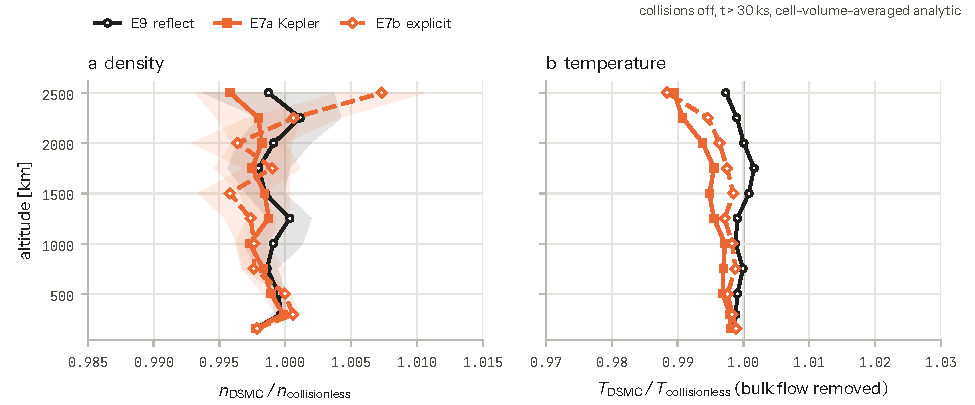
\includegraphics[width=\textwidth]{fig4_verification.pdf}
  \caption{Collisionless verification at $\rtop = $ \verZtopKm{}~km. Time-mean DSMC density (a) and bulk-flow-corrected temperature (b) over $t > $ \verTzero{}~ks, each divided by the cell-averaged collisionless solution for its UBC. E9 reflect is charcoal, E7a Kepler hold solid orange with squares, and E7b explicit RK4 dashed orange with diamonds. Bands are $\pm1$ standard error.}
  \label{fig:verif}
\end{figure}

\para{Against the collisionless solution} (Fig.~\ref{fig:verif}, Table~\ref{tab:verif}).
\begin{itemize}
  \item \textbf{Density.} The maximum $|\Delta n/n|$ is \verDnMaxKepler{}\% for E7a, \verDnMaxExplicit{}\% for E7b and \verDnMaxReflect{}\% for E9. The largest $|z|$ is \verZnMaxKepler{}, \verZnMaxExplicit{} and \verZnMaxReflect{}. These are sub-per-cent deviations made significant by very small batch-means errors.
  \item \textbf{Temperature.} The maximum $|\Delta T/T|$ is \verDTMaxKepler{}\%, \verDTMaxExplicit{}\% and \verDTMaxReflect{}\%.
  \item \textbf{Escape.} DSMC over analytic is \verEscRatioKepler{} ($k = $ \verEscKKepler{}, $z = $ \verEscZKepler{}), \verEscRatioExplicit{} ($k = $ \verEscKExplicit{}, $z = $ \verEscZExplicit{}) and \verEscRatioReflect{} ($k = $ \verEscKReflect{}, $z = $ \verEscZReflect{}).
  \item \textbf{Held inventory.} DSMC over the analytic $N_\mathrm{held}(t)$ is \verHeldRatioKepler{} for E7a and \verHeldRatioExplicit{} for E7b.
\end{itemize}

\para{Kepler hold against explicit RK4.}
\begin{itemize}
  \item E7a and E7b densities agree to max $|z| = $ \verKvsEZ{}, and their held counts differ by \verKvsEHeld{}\%.
  \item The RK4 return lags the Kepler prediction by \verDelayMean{}\,$\pm$\,\verDelayStd{}~s (Fig.~\ref{fig:time}f). For comparison, $\Delta t/2 = $ \verHalfDt{}~s and $\Delta t/\sqrt{12} = $ \verDelayUniformStd{}~s. That is the mean and s.d. of a delay distributed uniformly over one step. The explicit mover detects re-entry at the end of the step in which it happens, so this lag is the expected discretisation and not an orbit error.
  \item Held particles in E7b reached up to \verRheldMax{}~km altitude.
  \item \textbf{Restart.} E7d (restarted) against E7b agrees to max $|z| = $ \verRestartZ{} in density, and to \verRestartHeld{}\% in held count. The hold state survives a restart.
\end{itemize}

\para{Bookkeeping.} The balance invariant holds with a maximum violation of \verViolMax{} computational particles in all \verNHoldRuns{} runs, including the \texttt{-fcheck=all} build. In E9, $n_\mathrm{in} = n_\mathrm{ret}$ in every interval.

\para{Bug 2 in one plot.} E8 runs the old Kepler hold of \texttt{main}. Its bookkeeping is self-consistent: the invariant holds. But it records \eightReturns{} returns in \eightTend{}~s of simulated time:
\begin{itemize}
  \item The held count grows linearly, at \eightGrowth{} computational particles~\sinv{}, the entry rate after the first (spin-up) interval (\eightEntrySteady{}~\sinv{}; \eightEntry{}~\sinv{} including it).
  \item It ends at \eightHeldEnd{}, which equals the cumulative entries.
\end{itemize}
In other words, every particle that entered the hold stayed there (Fig.~\ref{fig:time}e). With the diagnostic in place, this frozen hold shows in the first interval as $n_\mathrm{ret} = 0$ beside $n_\mathrm{in} > 0$. The density deficit it caused had previously been hard to attribute.

\begin{table}[t]
  \caption{Hold bookkeeping of the verification runs, in computational particles. “Viol.”: maximum violation of the balance invariant. “Esc dir/orb”: escapes at $v>v_\mathrm{esc}$ and by the Hill cutoff. “Delay”: RK4 minus Kepler return time (UBC~5 only), mean $\pm$ s.d. in s. “Esc $z$”: DSMC escape against the collisionless rate, in Poisson errors. For E9 reflect, “in” and “ret” count reflections.}
  \label{tab:verif}
  \footnotesize
  \setlength{\tabcolsep}{3.4pt}
  \begin{tabular*}{\textwidth}{@{\extracolsep{\fill}}l rrrrrrr r r@{}}
    \toprule
    Run & Intervals & Viol. & In & Ret & Esc dir & Esc orb & Held end & Delay [s] & Esc $z$ \\
    \midrule
    \tablebody{tables/tab_verification.tex}
    \bottomrule
  \end{tabular*}
\end{table}

% ================================================================== 5
\section{Escape against domain size (Fig.~1 analogue)}\label{sec:escape}

\begin{figure}[t]
  \centering
  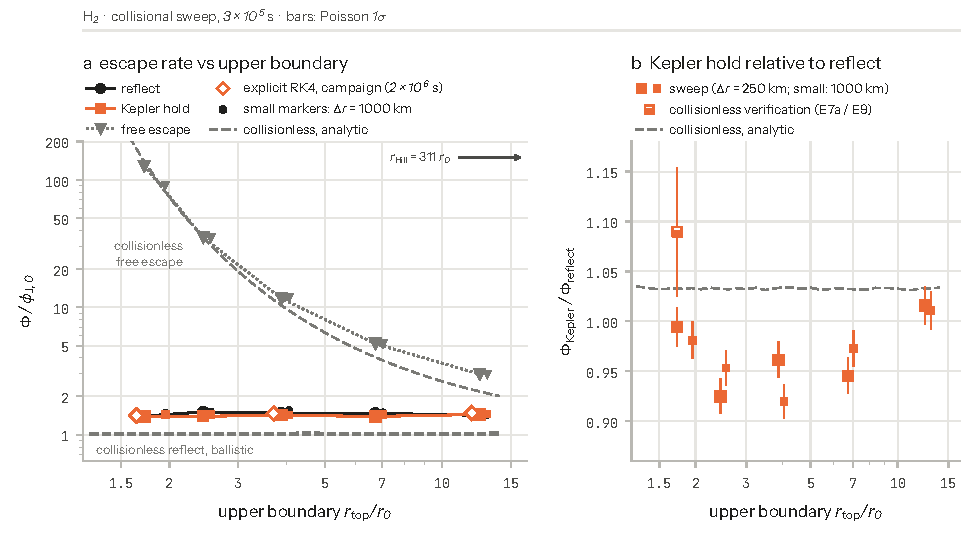
\includegraphics[width=\textwidth]{fig1_escape_rtop.pdf}
  \caption{(a) Escape rate $\Phi/\phi_{\mathrm{J},0}$ against $\rtop/r_0$ for the h2\_ubc\_rtop sweep, the analogue of Fig.~1 of \citet{cm21}. Large markers are $\Delta r = $ 250~km and small hollow markers $\Delta r = $ 1000~km. Grey dashed and dotted curves are the collisionless rates. The arrow points to $\rhill$, which lies off the axis. Hollow diamonds are the explicit RK4 runs of the \campTend{}~s campaign, averaged over their own steady windows; explicit RK4 is not part of the sweep. (b) $\Phi_\mathrm{Kepler}/\Phi_\mathrm{reflect}$ over the common steady window of each pair, with Poisson $1\sigma$ errors. The hollow square at the left is the collisionless E7a/E9 pair. The dashed line is the collisionless ratio, which exceeds unity only because of the Hill cutoff.}
  \label{fig:escape}
\end{figure}

\para{Rates} (Fig.~\ref{fig:escape}a, Table~\ref{tab:sweep}).
\begin{itemize}
  \item \textbf{Range.} Over all sweep runs, $\Phi/\phi_{\mathrm{J},0}$ is \phiOverJReflect{} for reflect, \phiOverJKepler{} for the Kepler hold and \phiOverJFree{} for free escape.
  \item \textbf{Collisionless rates.} At the top boundary these are \anReflectOverJ{} (reflect), \anBallisticOverJ{} (ballistic) and \anFreeOverJTop{} (free escape).
  \item \textbf{Collisions raise escape.} At \profZtop{}~km, reflect escapes \collEnhanceTop{} times the collisionless rate. The exobase lies above $r_0$, so the effective source is larger than the lower boundary, at nearly the same temperature (Table~\ref{tab:exo}).
  \item \textbf{Escape is steady in the window.} The window starts at \profWindowReflect{}~ks. Over the last third of each run ($t > $ \escLateStartKs{}~ks), escape differs from the window mean by \escDriftLo{} to \escDriftHi{}\%, with no common sign. (An earlier version of this report started each window where the particle inventory stopped drifting, as early as a few tens of ks, where escape was still rising. The fixed late window removes that transient. The campaign still uses inventory windows, but there the transient is a small part of a \campTend{}~s run.) Over the last third, reflect gives $\Phi/\phi_{\mathrm{J},0} = $ \escLateReflectRange{}, and \escLateCollEnhanceTop{} times the collisionless rate at the top. $\Phi_\mathrm{Kepler}/\Phi_\mathrm{reflect}$ over the same span is \sweepPhiRatioLateRange{}.
\end{itemize}

\para{Comparison with their Fig.~1.}
\begin{itemize}
  \item \textbf{Reflect does not grow with $\rtop$.} In \citet{cm21}, reflect escape grows with $r_\mathrm{max}$, because more exosphere is available for collisions that induce escape. Ours shows no such growth. The spread across tops is comparable to the $\Delta r$ effect (up to \drEffectMax{}\% between pairs with the same actual top), as expected when the exosphere above our lowest top is already collisionless. At \drSkipZtop{}~km the solver extends the last cell further for $\Delta r = $ 1000~km than for 250~km (Table~\ref{tab:sweep}), so that pair compares two tops, not two resolutions, and is left out of the $\Delta r$ effect.
  \item \textbf{Free escape stays well above the others.} It falls from \phiOverJFreeLowZ{} at \phiOverJFreeLowZkm{}~km to \phiOverJFreeTop{} at the top. It can only meet the Kepler hold near $\rhill = $ \oHill{}\,$r_0$, far beyond our range. In their case $\rhill = $ \pHill{}\,$r_0$, inside the plotted range, so their free-escape curve meets UBC~(2) there.
\end{itemize}

\para{Kepler hold relative to reflect} (Fig.~\ref{fig:escape}b). $\Phi_\mathrm{Kepler}/\Phi_\mathrm{reflect}$ spans \sweepPhiRatioRange{} over all \nSweepPairs{} pairs; the largest Poisson pull from unity is \sweepPhiRatioPullMax{}$\sigma$.
\begin{itemize}
  \item \textbf{Intermediate tops.} The ratio is below unity. This is a Carberry-like suppression, but of a few per cent rather than tens.
  \item \textbf{Highest top.} It is \sweepPhiRatioTop{}, consistent with the collisionless \anBallisticExcess{}\% Hill excess.
  \item \textbf{Systematic floor.} The suppression at intermediate tops is of the same size as the $\Delta r$ effect. We therefore treat it as suggestive, not established: the quoted $\sigma$ are statistical only.
  \item \textbf{The collisional campaign shows no larger suppression.} Over the steady windows of the \campTend{}~s runs, $\Phi_\mathrm{ballistic}/\Phi_\mathrm{reflect}$ is \campPhiRatioRange{} for both ballistic UBCs at the three tops (largest pull \campPhiRatioPullMax{}$\sigma$, \S\ref{sec:time}).
\end{itemize}

\begin{table}[t]
  \caption{Escape in the h2\_ubc\_rtop sweep. $t_0$: start of the averaging window (fixed, from the h2\_ubc\_rtop analysis). $k$: escaping computational particles counted in it. $\Phi/\phi_{\mathrm{J},0}$: $\pm$ Poisson $1\sigma$. “Coll.-less”: collisionless rate for the same UBC and $\rtop$. $\rtop/r_0$ is the actual top; at $z_\mathrm{top} = $ \drSkipZtop{}~km it differs between the two $\Delta r$.}
  \label{tab:sweep}
  \footnotesize
  \setlength{\tabcolsep}{3.8pt}
  \begin{tabular*}{\textwidth}{@{\extracolsep{\fill}}l rr r r r r r r@{}}
    \toprule
    UBC & $z_\mathrm{top}$ [km] & $\Delta r$ [km] & $\rtop/r_0$ & $t_0$ [ks] & $k$ & $\Phi$ [\sinv{}] & $\Phi/\phi_{\mathrm{J},0}$ & Coll.-less \\
    \midrule
    \tablebody{tables/tab_escape_sweep.tex}
    \bottomrule
  \end{tabular*}
\end{table}

% ================================================================== 6
\section{Profiles and exobase (Fig.~2 and Table~1 analogues)}\label{sec:profiles}

\begin{figure}[t]
  \centering
  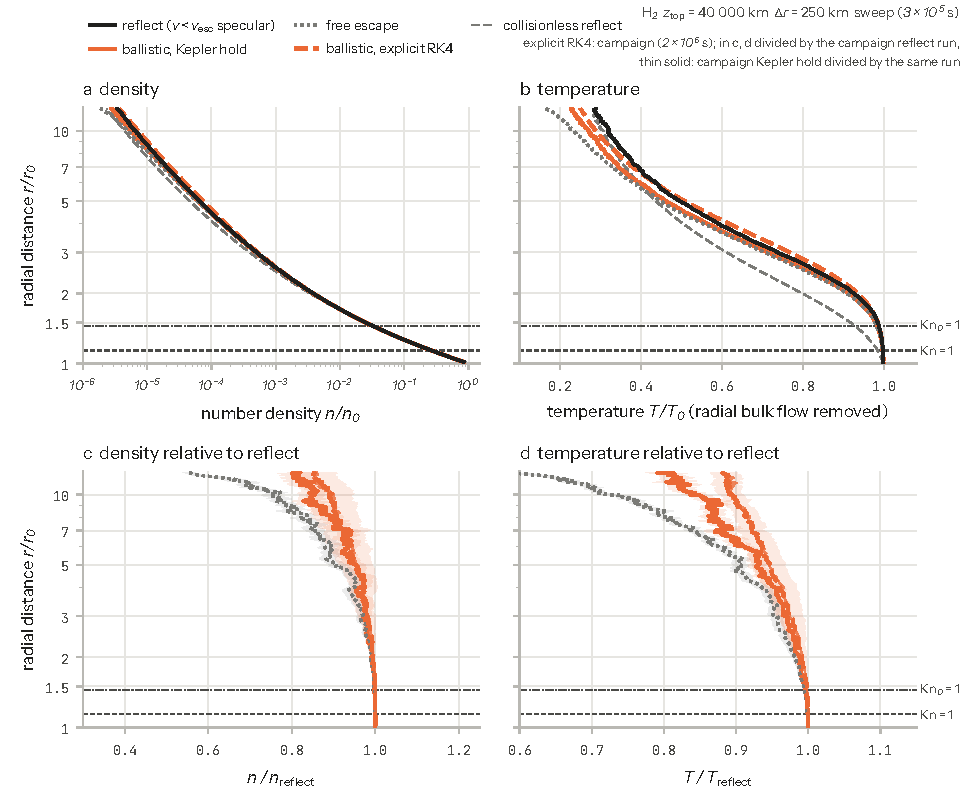
\includegraphics[width=\textwidth]{fig2_profiles.pdf}
  \caption{Time-mean profiles at $z_\mathrm{top} = $ \profZtop{}~km, $\Delta r = $ 250~km, from the sweep (\profWindowReflect{}~ks to \sweepTend{}~s), the analogue of Fig.~2 of \citet{cm21}. (a) $n/n_0$. (b) $T/T_0$ with the radial bulk flow removed. (c, d) The same, divided by reflect, with $\pm1\sigma$ bands. Horizontal lines: Kn\,=\,1 (dashed) and $\mathrm{Kn}_0$\,=\,1 (dash-dotted). Grey dashed: collisionless reflect. Explicit RK4 (dashed orange) comes from the \campTend{}~s campaign. In (c, d) it is divided by the campaign reflect run, and the thin solid orange line is the campaign Kepler hold divided by the same run, its like-for-like partner. Its distance from the thick (sweep, \sweepTend{}~s) Kepler curve is the further filling of the hold between \sweepTend{} and \campTend{}~s, not a difference between the two ballistic UBCs.}
  \label{fig:profiles}
\end{figure}

\para{Ballistic against reflect} (Fig.~\ref{fig:profiles}). At the top, the Kepler-hold exosphere is less dense and cooler than reflect:
\begin{itemize}
  \item \textbf{Density.} $n_\mathrm{Kepler}/n_\mathrm{reflect} = $ \nRatioKeplerTop{} at \profTopAltKm{}~km. The largest deviation is \nRatioKeplerMaxDev{}\%, at largest $|z|$ \nZmaxKepler{}, smaller than in $T$.
  \item \textbf{Temperature.} $T_\mathrm{Kepler}/T_\mathrm{reflect} = $ \TRatioKeplerTop{}, with largest deviation \TRatioKeplerMaxDev{}\% and largest $|z|$ \TZmaxKepler{}.
  \item \textbf{Free escape} is lower still: $n$ ratio \nRatioFreeTop{} ($|z|\le$ \nZmaxFree{}) and $T$ ratio \TRatioFreeTop{} ($|z|\le$ \TZmaxFree{}).
  \item \textbf{Reflect at the top} reaches $T = $ \TtopReflect{}~K, or \TtopReflectRaw{}~K without the bulk-flow correction.
  \item \textbf{Below $\mathrm{Kn}_0$\,=\,1}, all ratios are 1 within \belowKnZeroMaxDev{}\%.
\end{itemize}
This is the pattern of their Fig.~2. Reflection keeps an artificially full, warm population of slow particles near the top, whereas the Kepler hold is still filling: \heldFracSweepEnd{}\% of steady state at \sweepTend{}~s. Unlike their case, the perturbed region is collisionless, and the profile change does not feed back on escape (\S\ref{sec:escape}).

\para{Explicit RK4} (campaign, \campTend{}~s). Explicit and Kepler profiles agree. At the same run length, explicit/Kepler is \nRatioExplicitTop{} in $n$ and \TRatioExplicitTop{} in $T$ at the top, with max $|z|$ of \nZmaxExplicit{} and \TZmaxExplicit{} over the column, the same level as E7a/E7b (\verKvsEZ{}). Against the campaign reflect run, both ballistic UBCs are closer to reflect in $T$ at \campTend{}~s than the sweep Kepler hold is at \sweepTend{}~s: at the top, $T$ ratio \TRatioCampKeplerTop{} (Kepler) and \TRatioCampExplicitTop{} (explicit), against \TRatioKeplerTop{}. The $n$ ratios, \nRatioCampKeplerTop{} and \nRatioCampExplicitTop{} against \nRatioKeplerTop{}, are not significantly different. The reflect-induced warm excess shrinks as the hold fills.

\begin{table}[t]
  \caption{Exobase quantities per UBC at $z_\mathrm{top} = $ \profZtop{}~km, the analogue of Table~1 of \citet{cm21}. The Kn\,=\,1 exobase uses $\ell/H$ from the solver, and the $\mathrm{Kn}_0$\,=\,1 exobase uses $\ell/r_0$. Values are normalised to the source; $\phi_{\mathrm{J},x}$ is the Jeans rate at the exobase. An asterisk would mark an exobase in the bottom cell. Their profiles are taken after about one orbit, ours at \sweepTend{}~s (explicit RK4: campaign, \campTend{}~s).}
  \label{tab:exo}
  \footnotesize
  \setlength{\tabcolsep}{4pt}
  \begin{tabular*}{\textwidth}{@{\extracolsep{\fill}}l l r r r r r r r@{}}
    \toprule
    UBC & Definition & $z_x$ [km] & $r_x/r_0$ & $n_x/n_0$ & $T_x/T_0$ & $\lambda_x/\lambda_0$ & $\phi_{\mathrm{J},x}/\phi_{\mathrm{J},0}$ & $\Phi/\phi_{\mathrm{J},x}$ \\
    \midrule
    \tablebody{tables/tab_exobase.tex}
    \bottomrule
  \end{tabular*}
\end{table}

\para{Exobase} (Table~\ref{tab:exo}).
\begin{itemize}
  \item \textbf{Our exobase does not move with the UBC.} It is at \exoZReflectKn{}, \exoZKeplerKn{}, \exoZFreeKn{} and \exoZExplicitKn{}~km (Kn\,=\,1) for reflect, Kepler hold, free escape and explicit RK4. On the $\mathrm{Kn}_0$ definition it is at \exoZReflectKnZero{}, \exoZKeplerKnZero{}, \exoZFreeKnZero{} and \exoZExplicitKnZero{}~km.
  \item \textbf{The column is isothermal up to it}, with $T_x/T_0 = $ \exoTReflectKn{}.
  \item \textbf{In \citet{cm21} the Kn\,=\,1 exobase moves by several $r_0$.} It is \pExoKnReflect{}\,$r_0$ for reflect and \pExoKnBallistic{}\,$r_0$ for ballistic, against \pExoKnZeroReflect{}\,$r_0$ on the $\mathrm{Kn}_0$ definition. Their exobase lies inside the region the UBC perturbs. Ours does not.
\end{itemize}

\para{DSMC escape against Jeans at the exobase.} $\Phi/\phi_{\mathrm{J},x}$ (Kn\,=\,1) is \exoPhiReflectKn{} (reflect), \exoPhiKeplerKn{} (Kepler), \exoPhiExplicitKn{} (explicit) and \exoPhiFreeKn{} (free escape). Jeans at the exobase therefore underestimates escape only modestly for the two physical UBCs. For \citet{cm21}, the escape rate after about one orbit is \pPhiOneTorbReflect{}~\sinv{} for UBC~(1) and \pPhiOneTorbBallistic{}~\sinv{} for UBC~(3), a ratio of \pPhiOneTorbRatio{}. A strongly collisional exosphere drives non-Jeans escape that a column this rarefied does not have.

% ================================================================== 7
\section{Hold filling and the ballistic/return ratio (Fig.~3 analogue)}\label{sec:time}

\begin{figure}[p]
  \centering
  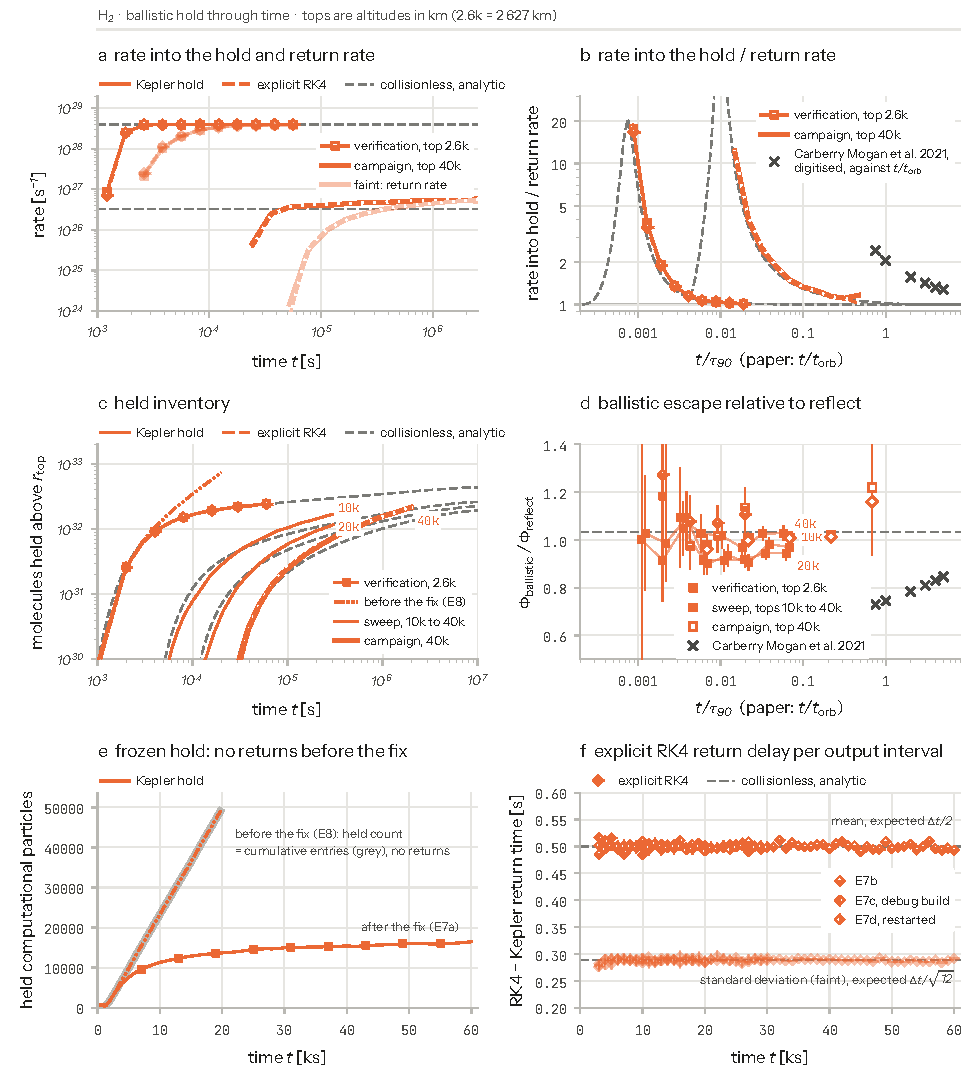
\includegraphics[width=\textwidth]{fig3_hold_time.pdf}
  \caption{Time dependence of the ballistic hold, the analogue of Fig.~3 of \citet{cm21}.
  (a) Rate into the hold (solid) and return rate (faint). Markers: verification ($\rtop = $ \verZtopKm{}~km, no collisions). Lines: campaign at $z_\mathrm{top} = $ \profZtop{}~km, with collisions, to \campTend{}~s. Dashed: collisionless $R_\mathrm{in}$.
  (b) Ballistic rate over return rate against $t/\tauf$, with collisionless curves for the two tops. Crosses: \citet{cm21}, digitised, plotted against $t/\torb$.
  (c) Held inventory: E7a, E7b and E8, the sweep Kepler hold at three tops, the campaign at \profZtop{}~km, and the collisionless $N_\mathrm{held}(t)$.
  (d) $\Phi_\mathrm{ballistic}/\Phi_\mathrm{reflect}$ against $t/\tauf$ for the sweep, verification and campaign. Crosses: \citet{cm21} against $t/\torb$.
  (e) E8 (\texttt{main}, bug~2): the held count equals cumulative entries, against the fixed E7a.
  (f) RK4 minus Kepler return delay per interval (E7b, E7c, E7d). Orange: mean, against $\Delta t/2$. Grey: s.d., against $\Delta t/\sqrt{12}$.}
  \label{fig:time}
\end{figure}

\begin{table}[t]
  \caption{Collisionless characteristic times per upper boundary (\texttt{dsmclib.exosphere}). $N_{\mathrm{held},\infty}$: steady held inventory (molecules). $R_\mathrm{in}$: rate of bound crossings into the hold. $\tauf$: time to 90\% of $N_{\mathrm{held},\infty}$ from empty. $t_\mathrm{ret,max}$: return time of the radial orbit with apoapsis at $\rhill$. “Excess”: collisionless ballistic over reflect escape, minus one.}
  \label{tab:times}
  \footnotesize
  \begin{tabular*}{\textwidth}{@{\extracolsep{\fill}}rr r r r r r r@{}}
    \toprule
    $z_\mathrm{top}$ [km] & $\rtop/r_0$ & $N_{\mathrm{held},\infty}$ & $R_\mathrm{in}$ [\sinv{}] & $\tauf$ [s] & $\tauf/\torb$ & $t_\mathrm{ret,max}$ [s] & Excess [\%] \\
    \midrule
    \tablebody{tables/tab_timescales.tex}
    \bottomrule
  \end{tabular*}
\end{table}

\para{Which clock.} Their Fig.~3 runs from \pFigThreeTlo{} to \pFigThreeThi{}\,$\torb$, and $\torb$ is a physical deadline for Callisto. Our natural clock is the hold's own fill time. $\tauf$ is \tauFillLo{}–\tauFillHi{}~s (\tauFillLoOrb{}–\tauFillHiOrb{}\,$\torb$), and the steady hold contains \heldSteadyLo{}–\heldSteadyHi{} molecules (Table~\ref{tab:times}). Measured in $\tauf$, our runs sit far to the left of theirs: the sweep reaches \sweepTendOverTau{}\,$\tauf$ and the campaign \campTendOverTau{}\,$\tauf$ at the highest top. Figs.~\ref{fig:time}b and d therefore share one axis with two meanings ($t/\tauf$ for us, $t/\torb$ for them); the curves do not overlap.

\para{Hold filling} (Fig.~\ref{fig:time}c).
\begin{itemize}
  \item \textbf{Collisionless runs.} E7a and E7b follow the collisionless $N_\mathrm{held}(t)$ (ratios \verHeldRatioKepler{} and \verHeldRatioExplicit{}).
  \item \textbf{Collisional sweep.} The Kepler-hold runs hold \sweepHeldOverAnalytic{} times the collisionless curve. That is of the same order as the collisional enhancement of the effective source seen in escape (\collEnhanceTop{}, \S\ref{sec:escape}).
  \item \textbf{Collisional campaign.} At \campTend{}~s, the held count (Kepler / explicit) is \campHeldOverAnalyticTop{} times the collisionless curve at \campZTop{}~km, \campHeldOverAnalyticMid{} at \campZMid{}~km and \campHeldOverAnalyticLow{} at \campZLow{}~km; the collisionless hold is then \campHeldFracAnTop{}, \campHeldFracAnMid{} and \campHeldFracAnLow{}\% full. At the two higher tops the enhancement is larger than in the sweep at \sweepTend{}~s (\sweepHeldOverAnalytic{}); at \campZLow{}~km, where the collisionless hold is nearly full, it falls within the sweep range. A likely reason, not tested here, is that the slow orbits that dominate the late inventory come from the same collisionally enhanced source above the exobase. Both ballistic UBCs give the same inventory.
\end{itemize}

\para{Ballistic/return ratio} (Fig.~\ref{fig:time}a, b).
\begin{itemize}
  \item \textbf{Analytic expectation.} Collisionless theory gives $R_\mathrm{in} = $ \anRinVer{}~\sinv{} at the verification top. The ratio $R_\mathrm{in}/(R_\mathrm{in} - \mathrm{d}N_\mathrm{held}/\mathrm{d}t)$ spikes before the first returns, then decays to \anInRetVerEnd{} by \verTend{}~s.
  \item \textbf{DSMC.} E7a and E7b give \verInRetKepler{} and \verInRetExplicit{} over $t > $ \verTzero{}~ks, matching theory, while the hold is only \heldFracVerEnd{}\% full.
  \item \textbf{Interpretation.} The long-period orbits hold many particles but carry little flux. The ratio therefore reaches unity long before the inventory does.
\end{itemize}
\citet{cm21} find instead \pInRetStart{} at \pFigThreeTlo{}\,$\torb$, still \pInRetEnd{} at \pFigThreeThi{}\,$\torb$.
\begin{itemize}
  \item \textbf{Collisional campaign.} Over $t > $ \campLateKs{}~ks, the ratio (Kepler / explicit) is \campInRetTop{} at \campZTop{}~km, \campInRetMid{} at \campZMid{}~km and \campInRetLow{} at \campZLow{}~km. The collisionless curve averaged over the same span gives \anInRetCampTop{}, \anInRetCampMid{} and \anInRetCampLow{}. Collisions below the top therefore barely change the ratio: it stays close to the collisionless value at each top, and well below theirs.
\end{itemize}

\para{Escape ratio} (Fig.~\ref{fig:time}d).
\begin{itemize}
  \item \textbf{Collisionless.} Verification gives $\Phi_\mathrm{ballistic}/\Phi_\mathrm{reflect} = $ \verPhiRatioKepler{} (Kepler) and \verPhiRatioExplicit{} (explicit), against the analytic \anPhiRatioVer{}.
  \item \textbf{Collisional sweep.} Over $t/\tauf \lesssim$ \sweepTendOverTau{}, the ratio stays within \sweepPhiRatioRange{}.
  \item \textbf{Collisional campaign.} Out to $t/\tauf = $ \campTendOverTau{}, over each run's steady window, it is \campPhiRatioRange{} for both ballistic UBCs at all three tops (largest pull \campPhiRatioPullMax{}$\sigma$). Longer runs do not open up a Carberry-size suppression.
  \item \textbf{Paper.} The digitised curve of \citet{cm21} rises from \pPhiRatioStart{} to \pPhiRatioEnd{}.
\end{itemize}

\subsection{Where we agree with Carberry Mogan et al., where we do not, and why}

\para{Agreement.}
\begin{itemize}
  \item A ballistic UBC leaves the upper exosphere less dense and cooler than reflection while the hold fills. The returning population is what reflection injects too early.
  \item The hold takes longer than any convenient run to reach steady state: here $\tauf$ exceeds both our run lengths and their $\torb$.
  \item Where the region perturbed by the UBC is collisional, ballistic escape falls below reflect. Our perturbed region is collisionless, and the few-per-cent suppression at intermediate tops is not established (\S\ref{sec:escape}).
\end{itemize}

\para{Disagreement 1: the size of the escape suppression.} Theirs is \pPhiRatioStart{}–\pPhiRatioEnd{}; ours is \sweepPhiRatioRange{}.
\begin{itemize}
  \item \textbf{Collisionality.} Their returning particles re-enter a region that is collisional out to an exobase at \pExoKnZeroReflect{}–\pExoKnReflect{}\,$r_0$. There they are scattered onto escape trajectories, so a missing return population directly removes escape. Our returns re-enter above an exobase at \exoRReflectKn{}\,$r_0$ and mostly fall through to the source without a collision.
  \item \textbf{Hill cutoff.} It adds a fixed \anBallisticExcess{}\% to ballistic escape, which partly offsets any suppression.
\end{itemize}

\para{Disagreement 2: the ballistic/return ratio.} Ours relaxes to unity early; theirs stays above unity for several $\torb$. We have three candidate causes. Our data cannot yet separate them.
\begin{itemize}
  \item \textbf{No Hill cutoff in their UBC~(3).} Return times diverge as $v \to v_\mathrm{esc}$, so a finite fraction of the inflow is always on orbits longer than the run. Our cutoff caps return times at \tReturnMax{}~s and removes that tail as escape.
  \item \textbf{Smaller $\lambda_{\mathrm{J},0}$} (\pLambdaZero{} against \oLambdaZero{}). This puts a larger share of the crossing flux close to escape speed, on long orbits.
  \item \textbf{Collisions above their exobase} can push particles onto near-escape orbits. In our collisionless verification this channel is absent by construction.
\end{itemize}
A collisionless calculation without the Hill cutoff at their $\lambda_{\mathrm{J},0}$ would test the first two (\S\ref{sec:open}).

\para{Disagreement 3: time normalisation.} Their $\torb$ is external to the gas. Our $\tauf$ is a property of the hold. Neither study's curves have converged, but for different reasons: theirs because the run is short against a heavy tail of return times, ours because the run is short against $\tauf$. In our runs the escape ratio is already near its asymptote while the hold inventory is not, so in this configuration escape converges much sooner than the inventory.

% ================================================================== 8
\section{Kepler hold against explicit tracking}\label{sec:kve}

\begin{figure}[t]
  \centering
  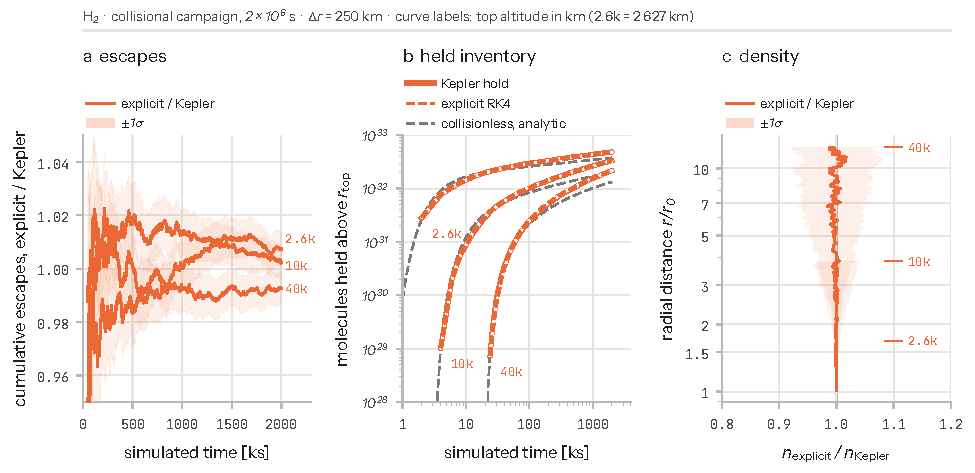
\includegraphics[width=\textwidth]{fig5_production.pdf}
  \caption{Explicit RK4 against the Kepler hold in the h2\_hold campaign (\campTend{}~s, collisions on), at each top; grey value marks the top. (a) Cumulative escapes, explicit/Kepler, with the Poisson $1\sigma$ band, from 50~ks on. (b) Molecules held above $\rtop$: Kepler solid, explicit dashed, collisionless $N_\mathrm{held}(t)$ grey dashed. (c) Time-mean density, explicit/Kepler, with $\pm1\sigma$.}
  \label{fig:prod}
\end{figure}

\para{Accuracy.} With point-mass gravity, the two UBCs are the same physics with the same escape decision.
\begin{itemize}
  \item \textbf{Verification} (\S\ref{sec:verif}): escape, held inventory and profiles agree within statistics. The only systematic difference is the sub-step lag of \verDelayMean{}~s. This is irrelevant for any process slower than $\Delta t$.
  \item \textbf{Collisional campaign} (\campTend{}~s, three tops; Fig.~\ref{fig:prod}, Table~\ref{tab:prod}). Explicit/Kepler escape is \prodEscRatioTop{} at the highest top. The time-mean held counts agree to \prodHeldRatioRange{}, and the density and temperature profiles to max $|z| = $ \prodZmaxN{} and \prodZmaxT{} over all tops, which is no more than the E7a/E7b verification pair (\verKvsEZ{}). The RK4 return delay keeps its $\Delta t/2$ value at every top (Table~\ref{tab:prod}), so collisions below $\rtop$ do not change the mover's behaviour above it. The hold balance closes exactly in every campaign run (largest violation \campViolMax{}), and in the reflect runs every interval has as many returns as entries (\campReflectInEqRet{}).
\end{itemize}

\para{Cost.} The Kepler hold still revisits each held particle every step to test its release time. Explicit tracking adds one RK4 push per held particle per step. Wall times (Kepler / explicit) are \prodWallKeplerTop{} / \prodWallExplicitTop{}~h at \campZTop{}~km, \prodWallKeplerMid{} / \prodWallExplicitMid{}~h at \campZMid{}~km and \prodWallKeplerLow{} / \prodWallExplicitLow{}~h at \campZLow{}~km, ratios of \prodWallRatioTop{}, \prodWallRatioMid{} and \prodWallRatioLow{}. The extra time grows with the number of held computational particles, which is largest at the lowest top (Fig.~\ref{fig:prod}b), so the ratio is largest there. Each run had a core of its own, but the machine was shared with other jobs, so differences of a few per cent are within the timing noise.

\begin{table}[t]
  \caption{Kepler hold (UBC~2) against explicit RK4 (UBC~5) in the h2\_hold campaign, \campTend{}~s with collisions. Ratios are explicit/Kepler: escapes over the whole run ($\pm$ Poisson), time-mean held count over the steady window, entries into the hold. $|z|_n$, $|z|_T$: largest profile $z$-score over the column. Delay: RK4 minus Kepler return time [s], mean $\pm$ s.d. over all returns. $z_\mathrm{held,max}$: highest altitude reached by a held particle [km]. Wall: hours, Kepler / explicit, and their ratio.}
  \label{tab:prod}
  \footnotesize
  \setlength{\tabcolsep}{3pt}
  \begin{tabular*}{\textwidth}{@{\extracolsep{\fill}}r r r r r r r r r r@{}}
    \toprule
    $z_\mathrm{top}$ [km] & Escape & Held & In & $|z|_n$ & $|z|_T$ & Delay [s] & $z_\mathrm{held,max}$ & Wall [h] & Ratio \\
    \midrule
    \tablebody{tables/tab_production.tex}
    \bottomrule
  \end{tabular*}
\end{table}

\para{When to use which.}
\begin{itemize}
  \item \textbf{Kepler hold (UBC~2)} is exact for two-body motion and independent of $\Delta t$. It needs no integration over orbits lasting up to \tReturnMax{}~s, which makes it the default for steady escape and structure runs under point-mass gravity.
  \item \textbf{Explicit tracking (UBC~5)} becomes necessary as soon as the motion above $\rtop$ is not Keplerian. Examples are solar tides near $\rhill$ (replacing the sharp cutoff), photo-destruction or ionisation in flight, rotation, or a multi-dimensional domain where the re-entry location matters. It also locates held particles in space ($r_\mathrm{held,max}$). Its RK4 error over the longest orbits has not been quantified separately. The verification orbits reach only \verRheldMax{}~km altitude; in the campaign held particles reach \campRheldMaxLo{}--\campRheldMaxHi{}~km with the return delay unchanged.
\end{itemize}

\para{Implications for gravity-wave runs.} \citet{cm21}, citing \citet{leclercq20}, argue that specular reflection washes out transients. A perturbation that reaches $\rtop$ is returned at once, as if the exosphere were in steady state. Both ballistic UBCs instead return it after the spread of orbital return times. Three implications follow for forced runs:
\begin{itemize}
  \item \textbf{Either ballistic UBC is appropriate}, and they give the same answer.
  \item \textbf{The spin-up is long.} The hold will still be filling, on $\tauf$, during any feasible wave run. The background therefore drifts slowly, and that drift must be detrended or the run started from a pre-filled hold (restart, \S\ref{sec:verif}).
  \item \textbf{$\rtop$ matters little for escape.} Here the escape rate is nearly independent of $\rtop$ under the Kepler hold. A lower top (shorter $\tauf$, cheaper) costs little accuracy in escape, but it truncates the region in which the wave can be observed.
\end{itemize}

% ================================================================== 9
\section{Limitations and next steps}\label{sec:open}

\begin{itemize}
  \item \textbf{The sweep has no hold diagnostics.} Sweep runs use the pre-diagnostic binary, so their in/return behaviour is not measured directly; the campaign measures it at three of the sweep's tops.
  \item \textbf{Two averaging windows.} Sweep values use the fixed \profWindowReflect{}~ks to end window of the h2\_ubc\_rtop analysis, campaign values the steady window of each run's inventory. Comparisons are made only within one group, except where a figure or sentence says otherwise.
  \item \textbf{None of the profiles is steady.} Every collisional profile describes a hold that is filling (\heldFracSweepEnd{}\% in the sweep, \heldFracCampEnd{}\% in the campaign at the highest top). The same holds for the profiles of \citet{cm21} after one orbit.
  \item \textbf{Resolution systematic.} The $\Delta r$ effect (up to \drEffectMax{}\% in escape at matched tops) is comparable to the Kepler/reflect differences at intermediate tops.
  \item \textbf{One seed per configuration.} The explicit/Kepler agreement is tested against Poisson and batch-means errors, not against seed-to-seed scatter.
  \item \textbf{The paper values are digitised.} Their Fig.~3 curves and Table~1 exobase radii are read by eye, and the parsed Table~1 is partly garbled. Only text-stated or legible values are used.
  \item \textbf{Weight.} \texttt{EXPERIMENT\_DESIGN.md} of the sweep quotes a different \Htwo{} particle weight. The run files and the campaign diagnostics agree on \oWeight{}, which is used throughout.
  \item \textbf{Next steps.}
    \begin{itemize}
      \item Compute the collisionless ballistic/return ratio with no Hill cutoff at $\lambda_{\mathrm{J},0} = $ \pLambdaZero{}, to test disagreement~2.
      \item Run one collisional configuration at Carberry Mogan's $\mathrm{Kn}_0$ (raise $n_0$ or lower the source altitude) with UBC~1, 2 and 5, to reproduce the size of their suppression.
      \item Run the sweep tops the campaign does not cover on the new binary, to complete the collisional in/return series.
    \end{itemize}
\end{itemize}

% ================================================================== references
\begin{thebibliography}{4}
\small
\bibitem[Carberry Mogan et al.(2021)]{cm21}
Carberry Mogan, S.R., Tucker, O.J., Johnson, R.E., 2021. The influence of upper boundary conditions on molecular kinetic atmospheric escape simulations. Planet.\ Space Sci.\ 205, 105302. \texttt{doi:10.1016/j.pss.2021.105302}.

\bibitem[Leclercq et al.(2020)]{leclercq20}
Leclercq, L., Williamson, H.N., Johnson, R.E., Tucker, O.J., Tian, L., Snowden, D., 2020. Molecular kinetic simulations of transient perturbations in a planet's upper atmosphere. Icarus 335, 113394.

\bibitem[Merryfield and Shizgal(1994)]{merryfield94}
Merryfield, W.J., Shizgal, B.D., 1994. Discrete velocity model for an escaping single-component atmosphere. Planet.\ Space Sci.\ 42 (5), 409–419.

\bibitem[Volkov et al.(2011)]{volkov11}
Volkov, A.N., Tucker, O.J., Erwin, J.T., Johnson, R.E., 2011. Kinetic simulations of thermal escape from a single component atmosphere. Phys.\ Fluids 23 (6), 066601.
\end{thebibliography}

{\small\color{graphite} \citet{merryfield94} calculated analytically the delay after which sub-escape particles re-enter through the upper boundary, which is the idea behind the Kepler hold. \citet{volkov11} used specular reflection to shorten the time to steady state. Both treatments ignore collisions above the boundary, so their steady states can agree \citep{cm21}, which is why reflection has been the default.}

% ================================================================== appendices
\appendix
\renewcommand{\thesection}{\Alph{section}}
\renewcommand{\thefigure}{\Alph{section}\arabic{figure}}
\renewcommand{\thetable}{\Alph{section}\arabic{table}}
\setcounter{figure}{0}
\setcounter{table}{0}

\section{Pipeline and provenance}\label{app:pipeline}

\para{Solver commits} (branch \texttt{feature/ubc-hold-explicit}, draft PR~\#14 on \#13).
\begin{itemize}
  \item \texttt{1c2c1a60}: E1–E6 experiments confirming the UBC fixes of \#13.
  \item \texttt{1206efc6}: the per-interval ballistic-hold diagnostic (in / return / escape counts).
  \item \texttt{43064c24}: UBC~5, explicit RK4 tracking of ballistic particles above $\rtop$.
  \item \texttt{0272e60d}: E7–E9 hold diagnostics and explicit-tracking verification.
\end{itemize}

\para{Binaries.}
\begin{itemize}
  \item \textbf{Verification:} \texttt{DSMC}, \texttt{DSMC\_dbg} and \texttt{DSMC\_mainA} in \texttt{\~{}/MarsAtmos-UBC-explicit/}, as listed per run in \texttt{verification/experiments.tsv}. \texttt{DSMC\_dbg} is the \texttt{-fcheck=all} build. \texttt{DSMC\_mainA} is the pre-fix Kepler hold of \texttt{main} (E8).
  \item \textbf{Sweep:} \texttt{\~{}/MarsAtmos-H2UBC-sweep/DSMC} at \texttt{64f21a1a}.
  \item \textbf{Campaign:} \texttt{\~{}/MarsAtmos-H2Hold-campaign/DSMC} at \texttt{43064c24} (\texttt{DSMC.commit}).
\end{itemize}

\para{Data tiers} (\texttt{refactored/docs/CONVENTIONS.md} 1.0).
\begin{itemize}
  \item \textbf{Raw:} the run folders, including \texttt{Results/Diagnostics/*\_BallisticHold.ascii}. Registry campaigns \texttt{h2\_hold} (E7a–E9 and \texttt{Hold\_H2\_U\{1,2,5\}\_z*\_dr250}) and \texttt{h2\_ubc\_rtop}.
  \item \textbf{Run:} \texttt{Results/<alias>\_run.nc}, built by \texttt{python -m dsmclib.runfile}.
  \item \textbf{Analysis:}\\ \texttt{outputs/h2\_hold/analysis/} (per run, and \texttt{h2\_hold\_analysis.nc} with the collisionless references and verification metrics), written by\\ \texttt{campaigns/h2\_hold/compute\_analysis.py};\\ \texttt{outputs/h2\_ubc\_rtop/analysis/}, written by\\ \texttt{campaigns/h2\_ubc\_rtop/compute\_analysis.py}.\\ Each file lists its source files and their SHA-256; the BallisticHold series is traced by count and a combined SHA-256.
  \item \textbf{Solver constants:} the VHS parameters are parsed from \texttt{MOD\_Species.f90}.
\end{itemize}

\para{Report scripts} (read analysis files only).
\begin{itemize}
  \item \texttt{dsmclib}: \texttt{escape}, \texttt{profiles} (bulk-flow temperature correction), \texttt{exosphere} (collisionless references) and \texttt{convergence} (steady windows), used by the campaign scripts.
  \item \texttt{scripts/analysis.py}: loads the analysis files and holds the parameters of \citet{cm21}.
  \item \texttt{scripts/make\_numbers.py}: writes \texttt{numbers.tex}, \texttt{tables/*.tex} and \texttt{numbers\_status.json}. Every number in this report set in the monospaced face comes from those files.
  \item \texttt{scripts/make\_figures.py}: renders all figures, as vector PDF and 300-dpi PNG.
\end{itemize}

\para{Rebuild.} The commands are in this folder's \texttt{README.md}: the run files, both campaign analyses, then the three report steps.

\para{AI assistance.} Claude (Anthropic) assisted with the analysis code, the figures and the drafting of this report, under the author's direction. Every reported value is generated from the run outputs by the scripts named here.

\section{Numbers status}\label{app:status}

The numbers were generated at \generatedOn{}. \texttt{numbers\_status.json} records the status of each input run and its analysis file, and would list any value written as \pending{reason}.

\begin{table}[H]
  \caption{Input runs by group and status at generation time. “Live”: runs with hold diagnostics but no analysis file.}
  \label{tab:inputs}
  \small
  \begin{tabular*}{\textwidth}{@{\extracolsep{\fill}}l rrrrrr@{}}
    \toprule
    Group & Total & Complete & Running & Queued & Stale & Live \\
    \midrule
    \tablebody{tables/tab_inputs.tex}
    \bottomrule
  \end{tabular*}
\end{table}

Pending values at generation time: \nPending{}.

\end{document}
